\section{DISEÑO DE INVESTIGACIÓN}
%http://recipp.ipp.pt/bitstream/10400.22/136/3/KDD-CRISP-SEMMA.pdf
%http://www.oldemarrodriguez.com/yahoo_site_admin/assets/docs/Documento_CRISP-DM.2385037

Uno de los pilares básicos en el diseño de una investigación es indicar el camino que se va a seguir en esta. Para ello, vamos a utilizar la metodologia CRISP-DM. \citeA{IBMCRISP2012}

La metodologia CRISP-DM tiene como objetivo orientar los proyectos de minería de datos. 
\begin{itemize}
	\item Como metodologia: incluye descripciones de las fases normales de un proyecto, las tareas necesarias en cada una de las fases y una explicación de las relaciones entre las tareas.
	\item Como modelo de proceso: ofrece un resumen del ciclo vital de la minería de datos.
\end{itemize}

La metodologia CRISP-DM establece un proceso genérico para satisfacer los objetivos deseados y contemplar la realización de la vigilancia e inteligencia. Este proceso se divide en distintas etapas básicas. 

El ciclo de vida de CRISP-DM esta compuesto de seis fases. La secuencia de estas no es estricta, es mas, la mayoria de proyectos avanzan y retroceden entre fases si es necesario. En la figura \ref{fig:CicloCrispDM} se puede observar cada fase.

\begin{figure*}[h]
\centering
\caption{Fases del ciclo de vida de CRISP-DM. Recuperado de \protect\citeA{IBMCRISP2012}.}
 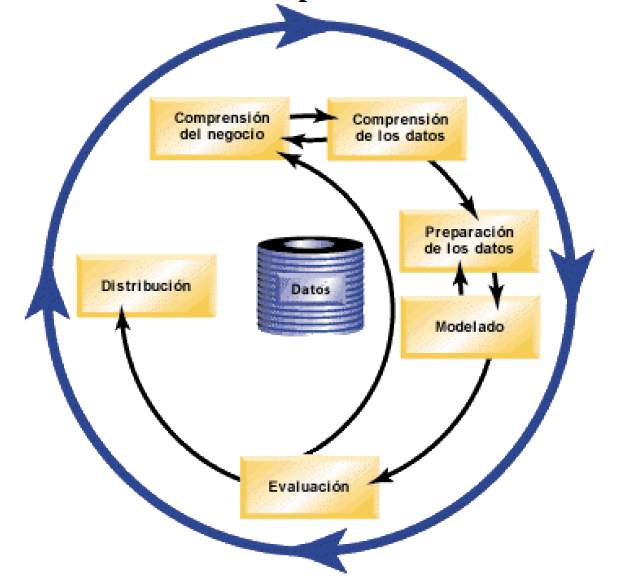
\includegraphics[width=0.6\textwidth]{recursos/CRISPCicloIBM}
\label{fig:CicloCrispDM}
\end{figure*}
\FloatBarrier

\begin{enumerate}
	\item Comprensión del negocio. Debe comprenderse los objetivos del negocio. Se debe realizar una descripción del problema. Por ultimo debe hacerse un plan de proyecto para alcanzar los objetivos deseados.
	\item Comprensión de los datos. Debe identificarse las fuentes de los datos y obtener aquellos datos relevantes para la consecución de los objetivos.
	\item Preparación de los datos. Conlleva el pre-procesado, la limpieza y la transformación de los datos relevantes con el objetivo de usar algoritmos de minería de datos.
	\item Modelado. Se debe desplegar un gran número de modelos y quedarse con aquellos que devuelvan valores óptimos para los datos utilizados.
	\item Evaluación. Debe evaluarse y probarse los modelos. Deben compararse entre sí y comprobar que son útiles para los datos expuestos.
	\item Distribución. Realizar actividades usando los modelos seleccionados en el proceso de la toma de decisión.
\end{enumerate}

En los próximos puntos se va a describir las actividades que se van a realizar en este proceso.

\subsection{Comprensión del negocio}
La primera tarea a realizar en el ciclo de CRISP-DM es obtener la máxima información posible de los objetivos de esta investigación.


\subsection{Comprensión de los datos}
Esta fase implica estudiar detalladamente los datos disponibles. Esta fase es esencial para evitar problemas inesperados durante la fase siguiente.

Para realizar esta fase, deberemos tener en cuenta dos consideraciones relacionadas. La primera consideración es la identificación de necesidades de informacion y la segunda es la identificacion de fuentes internas y externas.

\subsubsection{Identificación de necesidades de información}
Para realizar la identificación de las necesidades de información se va a partir de varios factores como son:
\begin{itemize}
	\item las demandas esperadas o manifestadas por (en este caso) una unidad de la consejería de educación.
	\item el análisis, la evolución de productos, procesos, materiales y tecnologías en el ámbito de la minería de datos educativa.
\end{itemize}
\subsubsection{Identificación de fuentes internas y externas de información}
Teniendo en cuenta las principales necesidades de información, se debe identificar las fuentes de información y recursos disponibles ya sean internos o externos a la organización. En este caso, se van a utilizar las siguientes fuentes:
\begin{itemize}
	\item Fundamentalmente se va a utilizar documentos y recursos internos de la organización como van a ser: repositorios documentales, carpetas locales, bases de datos, etc.
	\item Personas con conocimientos o experiencias relacionadas con la necesidad de información. En este aspecto se van a realizar distintas reuniones con las personas encargadas de esta unidad de la consejería de educación. Para ello se realizaran reuniones con estos responsables. A partir de estas reuniones se obtendrán las fuentes de información.
	\item Fuentes documentales a las que tiene acceso a la organización, ya sea en soporte físico (revistas, catálogos, etc.) como en soporte electrónico. Además, se utilizarán recursos de información en Internet (portales, noticias, redes sociales, foros, etc.). 
	\item Documentación técnica como reglamentaciones, especificaciones, propiedad industrial e intelectual o normas.
	\item Resultados de análisis existentes sobre las tendencias de futuro preferentemente en el ámbito educativo.
\end{itemize}

%\subsubsection{Búsqueda y tratamiento de la información}

La información fundamentalmente se encuentra en bases de datos internas, no obstante, se va a acceder a bases de datos externas en caso de necesidad para cumplimentar la información. 

En este aspecto, se debe recurrir a la ayuda de personas con conocimientos sobre el estado de las bases de datos. Como cualquier organización, la consejería de educación maneja grandes volúmenes de datos, por tanto, se debe tener conocimiento sobre donde se puede encontrar la información que satisfaga con las necesidades. 

El desconocimiento del estado de las bases de datos conlleva la inversión de una gran cantidad de tiempo en la búsqueda de los datos relevantes. 

%Una vez que se tienen los datos, muchas veces es necesario realizar un tratamiento de estos, que consiste en una limpieza y una normalización de los mismos. Muchas veces este tratamiento conlleva la conversión de datos, como por ejemplo fechas, corrección de datos, etc.

De esta fase se espera localizar todos los datos que posteriormente se prepararan y se utilizaran en el modelado.

\subsection{Preparación de los datos}
Una vez que se tienen claros los datos que se van a utilizar, se debe proceder a realizar la preparación para poder utilizarlos en la fase de modelado.

Algunas de las actividades que se van a realizar en esta fase son: la fusión de conjuntos y/o registros de datos, la selección de una muestra de un subconjunto, la agregación de registros, por contra la derivación de nuevos atributos a partir de anteriores, la eliminación o sustitución de valores en blanco o ausentes y por ultimo la división de datos de prueba y entrenamiento.

Ademas, también se va a estudiar la existencia de datos perdidos y errores en estos.

Para realizar este tratamiento de datos se utilizará la técnica conocida como ETL (extracción, transformación y carga) que consiste básicamente en obtener los datos de la fuente de origen (bases de datos, ficheros Excel, ficheros JSON, etc.), seleccionar aquellos datos que convengan al estudio, transformarlos según las necesidades que se tenga y depurarlos (evitando así datos erróneos). \cite{prakash2017etl} \cite{matos2006metodologia},\cite{gour2010improve}.
Para realizar este tratamiento, se ha va a utilizar Pentaho BI, que es un conjunto de programas libres para realizar entre otras muchas actividades, las técnicas de ETL. Concretamente, se ha utilizado la herramienta Spoon para desarrollar esta técnica. 
Una vez que se tienen los datos limpios y estructurados, se pueden realizar dos operaciones:

\begin{enumerate}
	\item  En primer lugar, se pueden almacenar dichos datos en una base de datos y seguir utilizando Pentaho BI para poder crear cuadros de mandos e informes. 
	\item  En segundo lugar, se puede almacenar la información en un texto plano para poder trabajar con herramientas de análisis descriptivo y predictivo. Estos análisis se van a realizar a través del entorno y lenguaje de programación R, que es una referencia en el ámbito de la estadística.
\end{enumerate}

\subsubsection{Análisis Exploratorio}

%El análisis predictivo (también conocido como estadísticas predictivas) se encarga de resumir los datos en bruto para que puedan ser interpretados. Estos análisis son útiles ya que permiten aprender sobre comportamientos o patrones pasados e entender cómo pueden influir en los resultados futuros. En este tipo de análisis se van a utilizar tanto métodos gráficos como medidas resumen.

En primer lugar, se debe estudiar el tipo de datos de cada variable a investigar, se debe clasificar las variables según sean categóricas (dicotómicas o polinómicas) o numéricas (discretos o continuos). El tipo de datos permite decidir qué tipo de análisis estadístico utilizar.
Una vez que se tienen claro el tipo de datos utilizados, se van a utilizar los principales estadísticos como la media, la mediana, las desviaciones típicas, etc.
Posteriormente se va a utilizar la matriz de varianzas y covarianzas, que indicaran la variabilidad de los datos y la información sobre las posibles relaciones lineales entre las variables. 

Por otro lado, se va a estudiar la correlación de las variables mediante la matriz de correlación. Esta matriz contendrá los coeficientes de correlación.\cite{JMMarin}. La matriz de correlación, se utilizará fundamentalmente por pares entre las variables y la variable a predecir.

También se va a estudiar la matriz de correlaciones parciales, que estudia la correlación entre pares de variables eliminando el efecto de las restantes.\cite{JMMarin}

Los datos categóricos se van a representar en tablas de frecuencias, gráficos de barras y gráficos de sectores. Los datos numéricos se van a representar mediante histogramas, boxplot y diagramas QQ-Plot o Grafico Cuantil-Cuantil. \cite{Orellana2001}

Mediante el boxplot se puede observar aspectos como la posición, dispersión, asimetría, longitud de colas y los datos anómalos (outliers). 
El QQ-plot se va a utilizar para evaluar la cercanía de los datos a una distribución. \cite{Orellana2001}

%(https://www.sergas.es/gal/documentacionTecnica/docs/SaudePublica/Apli/Epidat4/Ayuda/Ayuda_Epidat_4_Analisis_descriptivo_Octubre2014.pdf)
Por otro lado, se va a complementar el análisis descriptivo mediante el aprendizaje no supervisado, donde también se extraerán otras características de los datos.

%En este apartado, se va a presentar la forma en la que se va a realizar la investigación. En primer lugar, se va a realizar un proceso ETL, posteriormente se va a realizar un análisis descriptivo mediante sus técnicas que se explicaran posteriormente, además se va a incluir técnicas de aprendizaje no supervisada en este análisis.
%Una vez que se ha realizado el análisis descriptivo, se va a realizar un análisis predictivo. En este análisis se va a utilizar técnicas de aprendizaje supervisadas.


\subsection{Modelado}

\subsubsection{Modelos seleccionados}
Los métodos de predicción que se van a utilizar para resolver el problema en cuestión van a ser aquellos que mejores resultados han obtenido utilizando los datos de varias líneas de investigación estudiadas. Estos métodos son los siguientes: árboles de decisión, redes neuronales, k-vecinos cercanos, bosques aleatorios y regresión logística. Obviamente se debe destacar que, aunque se van a utilizar dichos métodos, pueden existir otros que se ajusten mejor a los datos.

\subsubsection{Aprendizaje automático}


%https://www.fisterra.com/mbe/investiga/10descriptiva/10descriptiva.asp#top
%http://www.uco.es/zootecniaygestion/img/pictorex/27_12_49_7.pdf
%https://machinelearningmastery.com/descriptive-statistics-examples-with-r/
%http://cms.dm.uba.ar/academico/materias/verano2015/estadisticaQ/descriptiva.pdf

\textbf{Aprendizaje Supervisado}

Una vez terminado el análisis descriptivo, se va a realizar un análisis predictivo. Se debe tener en cuenta, que, dentro de la ciencia de datos, existen técnicas de aprendizaje automáticas, cuyo objetivo es la construcción de un sistema que sea capaz de aprender a resolver problemas sin la intervención de un humano. \cite{MARIN2018}.

El aprendizaje supervisado consiste en la búsqueda de patrones en datos históricos relacionando todas las variables con una especial (conocida como variable objetivo). Los algoritmos que se utilizan en el aprendizaje supervisado se encarga de buscar patrones en los datos. A este proceso se conoce como entrenamiento de los datos. Una vez que se tienen los patrones, se aplican a los datos de prueba. Los datos de entrenamiento suelen ser una selección aleatoria y única de los datos históricos de un 70\% del total. Los datos de prueba son el restante 30\%. \cite{Manguart2017}.
Algunos de los algoritmos que se van a utilizar son:
\begin{enumerate}
	\item Arboles de decisión
	
	Se basa en el descubrimiento de patrones a partir de ejemplos. Un árbol de decisión está formado por un conjunto de nodos (de decisión) y de hojas (nodos-respuesta).
	
	Los nodos están asociados a los atributos y tiene varias ramas que salen de él (dependiendo de los valores que tomen la variable asociada). Estos nodos pueden asemejarse a preguntas que, dependiendo de la respuesta que conlleve, se tomara un flujo en las ramas salientes.
	
	Los nodos respuesta están asociados a la clasificación que se desea proporcionar, devolviendo así la decisión del árbol con respecto al ejemplo de entrada utilizado.
	
	\begin{figure*}[htb]
		\centering
		\caption{Funcionamiento Árboles Decisión. Recuperado de \protect\citeA{sayad2019}}
		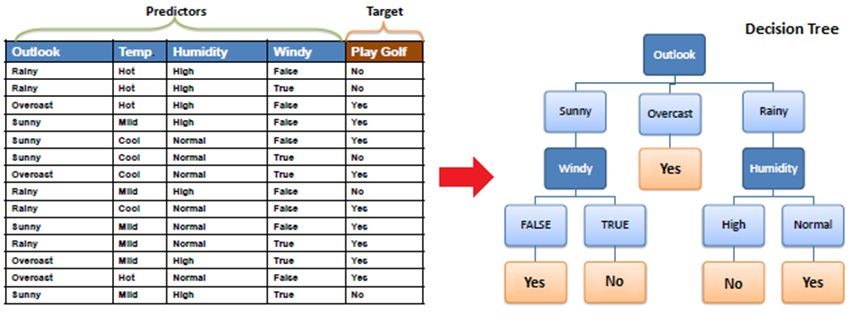
\includegraphics[width=0.8\textwidth]{recursos/arbol_decision_img1}
		\label{fig:fun_arb_dec}
	\end{figure*}
	\FloatBarrier
	
	
	\item Clasificación de Naïve Bayes.
	
	Es un algoritmo que se basa en la técnica de clasificación utilizando el teorema de Bayes.
	
	El algoritmo es capaz de agrupar un registro mediante las características de este. Para ello aplica probabilidades condicionales de las características para determinar a qué categoría pertenece. 
	
	Por ejemplo, una fruta puede considerarse una manzana si es de color rojo, redonda y tiene un determinado peso.
	
	\begin{figure*}[htb]
		\centering
		\caption{Teorema de Bayes. Recuperado de \protect\cite{uCincinnati2018}}
		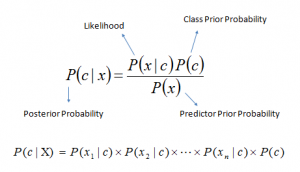
\includegraphics[width=0.6\textwidth]{recursos/BayesFormula}
		\label{fig:BayesFormula}
	\end{figure*}
	\FloatBarrier
	
	\item Regresión Logística
	
	Es un algoritmo de regresión que se utiliza para predecir el resultado de una variable categórica en función de las variables independientes o predictores. Para predecir el resultado, se establecen pesos en función de la puntuación dada a cada variable independiente.
	
	\item Redes Neuronales
	%https://www.tuinteligenciaartificial.es/las-redes-neuronales-en-la-inteligencia-artificial-explicacion-clara-y-sencilla/
	
	Las redes neuronales son un algoritmo de inteligencia artificial que se inspira en los mecanismos presentes en la naturaleza. Las neuronas envían señales eléctricas de manera fuerte o débil a otras neuronas. La combinación de todas las conexiones entre neuronas es lo que genera el conocimiento. Estas señales se envían cuando existe unos estímulos (inputs) externos a través de los sentidos. A lo largo de la vida, las neuronas aprenden que deben hacer a partir de dichos estímulos y, por lo tanto, los seres vivos aprenden a actuar ante distintas señales y situaciones. El funcionamiento de las redes neuronales en la inteligencia artificial es similar.
	
	\begin{figure*}[htb]
		\centering
		\caption{Red Neuronal. Recuperado de \protect\citeA{yepes2017}}
		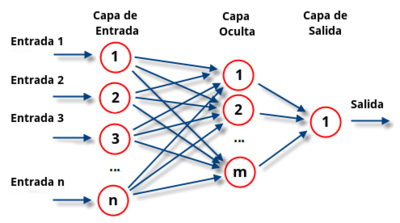
\includegraphics[width=0.6\textwidth]{recursos/RedNeuronalArtificial}
		\label {fig:RedNeuronal}
	\end{figure*}
	\FloatBarrier
	
	Como se puede observar en la figura \ref{fig:RedNeuronal}, la primera fila (con neuronas de color rojo), se conocen como nodos de entrada y son aquellos que se encargan de recoger la información. Los nodos en la gama azul son los que se conocen como nodos de salida. Los nodos situados en el medio son aquellos que se encargan de hacer el aprendizaje, y se conocen como nodos ocultos.
	
	En primer lugar, se obtiene la información a partir de los nodos de entrada, una vez que se tiene la información, se envía a las capas ocultas, que se activan o no dependiendo del aprendizaje previo. Los nodos ocultos se activan dependiendo de una serie del resultado de unas operaciones matemáticas. Si los nodos se activan, entonces enviaran la información a la siguiente capa.
	
	\item Bosques aleatorios
	
	Los bosques aleatorios son un método que se encarga de combinar los resultados de árboles de decisión independientes.
	
	Algunas características son:
	\begin{itemize}
		\item Gran precisión.
		\item Eficiente para grandes bases de datos.
		\item Aporta estimaciones sobre la importancia de las variables en la clasificación.
		\item Tiene un método eficaz para la estimación de los datos faltantes y mantiene la precisión cuando falta una gran parte de los datos.
	\end{itemize}
	%https://quantdare.com/random-forest-vs-simple-tree/
	%http://randomforest2013.blogspot.com/2013/05/randomforest-definicion-random-forests.html
	%https://bookdown.org/content/2031/ensambladores-random-forest-parte-i.html
	
	\item K-Vecinos-cercanos
	
	K-vecinos-cercanos (conocido también como K-NN) es un algoritmo de aprendizaje supervisado en el que, a partir de unos datos iniciales, es capaz de clasificar todas las nuevas instancias.
	
	La idea es que el algoritmo clasifica cada dato nuevo en el grupo que corresponda, según cual sea el grupo vecino (de los k grupos) mas próximo. Por tanto, calcula la distancia del elemento nuevo a cada uno de los existentes e indica a que grupo debe permanecer este nuevo elemento según la menor distancia.
	
	\begin{figure*}[htb]
		\centering
		\caption{KNN. Recuperado de \protect\citeA{klein2018}}
		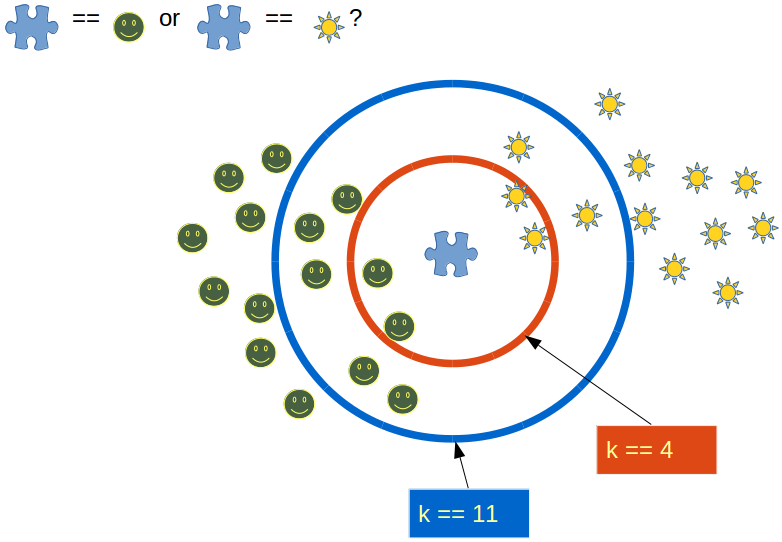
\includegraphics[width=0.6\textwidth]{recursos/k_NN}
		\label {fig:KNN}
	\end{figure*}
	\FloatBarrier
	
	
\end{enumerate}

\subsubsection{Criterio de selección}
Una vez que se han seleccionado las variables y los algoritmos a estudiar, es hora de realizar el propio modelado. Al realizar el modelado, deberemos tener en cuenta que variables son mejores para este modelado. Es posible que existan variables que únicamente empeoren los resultados del modelado, por lo tanto, se deberán desestimar. Para ello se va a utilizar el criterio de Akaike (AIC). 

Este criterio indica el ajuste que tienen los datos experimentales con el modelo utilizado. Obviamente, el criterio de AIC solo tiene sentido cuando se realizan comparaciones con otros modelos (utilizando el mismo conjunto de datos). \cite{martinez2009criterio}

Cuanto menor sea el valor de este criterio, mejor se ajustan los datos al modelo. Por tanto, se deberá seleccionar el modelo que menor AIC tenga. \cite{martinez2009criterio}

\subsection{Evaluacion}
\subsubsection{Métricas de precisión}
Las métricas que se va a utilizar para obtener la precisión de los modelos van a ser aquellas descritas en el artículo de  \citeA{COSTA2017247}, \citeA{Helal2018} y \citeA{ASHRAF20181021}. Estas métricas son frecuentes en ámbitos como la obtención de información, aprendizaje automático y otros dominios como la clasificación binaria. Dichas métricas van a ser las siguientes:

\begin{itemize}
	\item FMeasure: es la media armónica de la precisión y recuperación de un clasificador; es decir, FMeasure = 2 * Precision * Recall / (Precision + Recall).
	\item Precision: es la fracción de verdaderos positivos entre todos los ejemplos clasificados como positivos. P= TP/(FP+TP).
	\item Recall: es la fracción de verdaderos positivos clasificados correctamente. R = TP/(FN+TP).
	\item AUC: el área bajo la característica de operación del receptor. La curva (ROC) indica la probabilidad de que un clasificador clasifique un positivo seleccionado aleatoriamente sobre un negativo. Un AUC con valor de 1 indica un perfecto clasificador, mientras que 0.5 implica que el clasificador lo hace de forma aleatoria.
\end{itemize}

Donde:
\begin{itemize}
	\item TP - Verdadero Positivo: es el número de instancias positivas clasificadas correctamente como positivas. 
	\item FP - Falso Negativo: es el número de instancias positivas clasificadas incorrectamente como negativas.
	\item FP - Falso Positivo: es el número de instancias negativas clasificadas incorrectamente como positivas.
	\item TN - Verdadero Negativo: es el número de instancias negativas clasificadas correctamente como negativas.
\end{itemize}

Estas métricas se van a mostrar utilizando un gráfico conocido como matriz de confusión.


\subsection{Distribucion}
Respecto a la distribución de la información, esta no podrá salir de la consejería de educación. Aunque se trate de datos anonimizados y agregados, se trata de datos de carácter sensible y no pueden ser distribuidos. Por tanto, dichos datos se van a almacenar en un gestor de bases de datos MySQL. Este gestor se encontrará en un servidor de la Consejería de Educación. Solo se va a poder acceder a dicho servidor desde la propia sede. Es posible que los datos también se almacenen en archivos de texto plano.




